\documentclass[11pt,a4paper]{article}
\usepackage[utf8]{inputenc}
\usepackage[T1]{fontenc}
\usepackage[brazilian]{babel}
\usepackage{lmodern}
\usepackage[margin=2cm]{geometry}
\usepackage{graphicx}
\usepackage{booktabs}
\usepackage{float}
\usepackage{longtable}
\usepackage{array}
\usepackage[font=small,labelfont=bf]{caption}
\usepackage{xurl}
\usepackage[hidelinks]{hyperref}

\graphicspath{{../results/}{figuras/}}
\makeatletter
\newcommand{\linhas}[1]{\@@input #1 }
\setlength{\@fptop}{0pt}\setlength{\@fpsep}{14pt}\setlength{\@fpbot}{0pt plus 1fil}  % \input primitivo: o do LaTeX quebra dentro da longtable
\makeatother
\newcommand{\valFinal}{97,52\%}
\newcommand{\testeFinal}{97,89\%}
\newcommand{\valEnsCinco}{97,31\%}
\newcommand{\testeEnsCinco}{97,63\%}
\newcommand{\valCnnBest}{96,68\%}
\newcommand{\testeCnnBestFinal}{97,13\%}
\newcommand{\valLinear}{30,29\%}
\newcommand{\treinoLinear}{30,97\%}
\newcommand{\valMlp}{86,25\%}
\newcommand{\treinoMlp}{95,08\%}
\newcommand{\valMlpMelhor}{86,88\%}
\newcommand{\valMlpBnDropout}{86,46\%}
\newcommand{\valCnn}{95,33\%}
\newcommand{\treinoCnn}{99,24\%}
\newcommand{\valWtrinta}{96,98\%}
\newcommand{\valWsessenta}{96,86\%}
\newcommand{\valCftrinta}{96,68\%}
\newcommand{\valCfsessenta}{96,78\%}
\newcommand{\valEsessentaMedia}{96,72\%}
\newcommand{\difMlpBnDropout}{3,3}


\begin{document}

\begin{titlepage}
  \centering
  {\large Universidade Federal de Mato Grosso do Sul\par}
  \vspace{0.5cm}
  {\large Inteligência Artificial --- turma P03, 2026-2\par}
  \vspace{4cm}
  {\LARGE\bfseries Classificação de dígitos no dataset SVHN\par}
  \vspace{0.5cm}
  {\large Relatório do trabalho final\par}
  \vspace{3cm}
  {\large Samuel Vieira da Cunha Nahas\\
          Wilker Sebastian Afonso Pereira\\
          Bernardo Willian de Sousa Pereira\par}
  \vspace{2cm}
  {\large Professor: Wesley Nunes Gonçalves\par}
  \vfill
  {\large Novembro de 2026\par}
\end{titlepage}

\begin{abstract}
Este relatório descreve a classificação dos dígitos do SVHN com redes neurais em PyTorch, usando só os
conjuntos \texttt{train} e \texttt{test}. Partimos de um classificador linear (\valLinear{} de validação) e de
uma MLP (\valMlp{}) e chegamos a uma CNN de três blocos com data augmentation, cutout, weight decay e label
smoothing (\valCnnBest{}). Toda escolha foi feita pela validação, numa divisão fixa do \texttt{train} com a
semente 42. A solução final é um ensemble de 20 dessas CNNs, treinadas por 60 épocas com sementes fixas e
avaliadas com deslocamentos de 1 e 2 pixels (TTA). Ela tem \valFinal{} de validação e \testeFinal{} no teste,
e é o modelo que gerou as predições do conjunto adicional. As mudanças de maior impacto foram trocar a MLP pela
CNN, normalizar a entrada, usar data augmentation e combinar vários modelos.
\end{abstract}

\section{Solução desenvolvida}

\paragraph{Protocolo.} O \texttt{split="train"} (73.257 imagens) foi dividido em 90\% para treino (65.932) e
10\% para validação (7.325), sempre com a semente 42. A normalização usa a média e o desvio de cada canal
calculados só no treino. Cada modelo é avaliado na época de maior acurácia de validação. O \texttt{split="test"}
(26.032 imagens) só informa a acurácia e não participa de nenhuma escolha, e o conjunto adicional do professor
só foi usado depois que a solução final estava definida. Todos os modelos usam batch 64, taxa de aprendizado
com decaimento cosseno ao longo das épocas e entropia cruzada, salvo quando o próprio experimento muda isso.

\paragraph{Semente.} A semente 42 fixa a divisão treino/validação, a inicialização dos pesos, a ordem dos lotes
e o augment, de modo que rodar de novo dá o mesmo resultado e todos os experimentos são comparados nas mesmas
7.325 imagens de validação. No ensemble, o membro $i$ usa a semente $42+i$ (42 a 61), numa ordem fixada antes de
ver os resultados. A divisão continua sendo sempre a da semente 42.

\paragraph{Classificador linear.} Uma camada linear de $3\cdot32\cdot32 = 3072$ entradas para 10 saídas
(30.730 parâmetros), com softmax e entropia cruzada. Foi treinado com Adam, taxa de aprendizado $10^{-3}$, por 15
épocas. Também testamos a loss SVM multiclasse da aula.

\paragraph{MLP.} Duas camadas ocultas de 512 e 256 neurônios com ReLU (1.707.274 parâmetros), com as mesmas
condições do linear: Adam, taxa de aprendizado $10^{-3}$, batch 64 e 15 épocas. A partir dela variamos a taxa de
aprendizado, o batch, o otimizador (SGD, com e sem momentum), as ativações, a normalização da entrada, a
profundidade e a regularização (L2, Dropout e BatchNorm).

\paragraph{CNN.} Três blocos de convoluções $3\times3$ com BatchNorm e ReLU, seguidos de max pooling (32, 64 e
128 filtros; a imagem vai de $32\times32$ a $4\times4$), e uma camada densa de 256 com Dropout 0,3. Sobre ela
testamos data augmentation (rotação de $\pm8^\circ$, escala de $\pm10\%$ e translação de $\pm8\%$, sem
espelhamento, porque um dígito espelhado é outro símbolo), filtros mais largos, weight decay, mais épocas, label
smoothing, uma terceira convolução por bloco e cutout (um quadrado de $8\times8$ zerado em posição aleatória).

\paragraph{Hiperparâmetros mais importantes.} Pelos experimentos, os que mais pesaram foram a taxa de
aprendizado (com Adam, $10^{-2}$ impede o treino da MLP), a normalização da entrada, o data augmentation, o
número de épocas e, na solução final, o número de modelos do ensemble. Batch, ativação ReLU contra Leaky ReLU e
largura da CNN mudaram pouco.

\paragraph{Código.} O notebook \texttt{svhn.ipynb} tem o classificador linear, as MLPs, as CNNs, o ensemble de
5, a solução final e as predições. Os treinos em lote (as triagens sobre a \texttt{cnn\_best}, as confirmações com
várias sementes e os ensembles de 60 épocas) usaram o script \texttt{dgx/svhn\_dgx.py}, com o mesmo protocolo, a
mesma divisão e a mesma normalização do notebook. O script confere a divisão antes de treinar.

\paragraph{Organização e metodologia.} O trabalho foi feito no GitHub, em
\url{https://github.com/SamuelNahas/svhn-classificacao}, onde estão o código, os pesos, os resultados de cada
experimento e este relatório. Cada entregável virou uma issue, com as decisões do grupo registradas numa issue
principal, e o andamento foi acompanhado num board, em
\url{https://github.com/users/SamuelNahas/projects/2} (Backlog, Fazendo, Verificação e Pronto). Cada issue teve a
sua branch e um pull request revisado antes de entrar. A cada pull request, a integração contínua executa o
notebook inteiro num modo de teste rápido e confere as saídas. Nos experimentos, cada rodada mudou uma coisa
por vez, e o plano e a regra de decisão de cada rodada foram registrados no repositório antes de rodar.

\section{Experimentos}

A Tabela~\ref{tab:evol} segue o formato pedido: cada linha parte da anterior e diz o que foi alterado, o
resultado e se houve melhora ou piora em relação ao modelo anterior. A Tabela~\ref{tab:outros} traz os demais
experimentos, agrupados por família, cada um comparado ao modelo de que deriva. Todas as acurácias são da melhor
época de validação, e a escolha sempre foi feita pela validação. A Tabela~\ref{tab:outros} também traz a loss e a acurácia de treino de cada
experimento; as dos modelos da Tabela~\ref{tab:evol} estão na Tabela~\ref{tab:treino} (Seção~\ref{sec:curvas}).

\begin{table}[h]
\centering\small
\caption{Evolução até a melhor solução. Acurácias em \%. A última coluna compara a validação com a linha
anterior, em pontos.}\label{tab:evol}
\begin{tabular}{r>{\raggedright}p{2.8cm}>{\raggedright}p{5.6cm}rr>{\raggedright\arraybackslash}p{3.3cm}}
\toprule
\# & Experimento & Modificação & Validação & Teste & Em relação ao anterior \\
\midrule
\linhas{tabelas/evolucao.tex}
\bottomrule
\end{tabular}
\par\vspace{0.3em}
\begin{minipage}{0.97\textwidth}\footnotesize
$^a$ A validação da solução final é a do ensemble de 20 com TTA, com os membros treinados só no treino. Para
a predição, os mesmos 20 foram retreinados com todo o \texttt{split="train"}, cada um até a melhor época de
validação da sua semente, e é esse ensemble que tem o teste indicado. As linhas 7 a 10 são ensembles: a média do
softmax de modelos iguais com sementes diferentes.
\end{minipage}
\end{table}

{\small
\setlength{\tabcolsep}{3pt}
\begin{longtable}{>{\raggedright}p{6.9cm}rrrrr>{\raggedright\arraybackslash}p{2.9cm}}
\caption{Demais experimentos. Cada linha muda uma coisa em relação à base indicada. Loss: entropia cruzada.
Acurácias em \%. Ensembles não têm métricas de treino (---).}\label{tab:outros}\\
\toprule
 & \multicolumn{2}{c}{Loss} & \multicolumn{3}{c}{Acurácia} & \\
Modificação & treino & val. & treino & val. & teste & Em relação à base \\
\midrule
\endfirsthead
\toprule
 & \multicolumn{2}{c}{Loss} & \multicolumn{3}{c}{Acurácia} & \\
Modificação & treino & val. & treino & val. & teste & Em relação à base \\
\midrule
\endhead
\bottomrule
\endfoot
\linhas{tabelas/outros.tex}
\end{longtable}
}
\vspace{-0.8em}
{\footnotesize
$^b$ Treinos em lote: a loss e a acurácia de treino são medidas numa amostra fixa de 7.325 imagens do treino, e
a acurácia de teste foi calculada durante os treinos, mas só foi lida depois de a solução final estar fechada,
sem influenciar nenhuma escolha. \quad
$^c$ TTA $\pm2$\,px: a imagem e 4 cópias deslocadas 2 pixels; shift12: a imagem e 8 cópias deslocadas 1 e 2
pixels. Com shift12, o teste só foi calculado para a solução final (---).
\par}

\paragraph{O que os experimentos mostram.}
\begin{itemize}
  \item \textbf{Família de modelo.} Linear, MLP e CNN são os maiores saltos: \valLinear{}, \valMlp{} e \valCnn{}
        na validação. O linear sobre pixels crus não separa os dígitos, e a CNN ganha por aproveitar a estrutura
        espacial da imagem.
  \item \textbf{MLP.} A normalização é essencial (sem ela, a validação cai para menos de 50\%), a taxa de
        aprendizado $10^{-2}$ com Adam impede o treino, e tanh e sigmóide aprendem pior que ReLU. O SGD com
        momentum foi a melhor MLP (\valMlpMelhor{}). Dropout sozinho reduz a diferença entre treino e validação,
        mas perde acurácia; com BatchNorm, a acurácia volta e a diferença cai para cerca de 3 pontos.
  \item \textbf{CNN.} Data augmentation, weight decay, 30 épocas, label smoothing, a terceira convolução por bloco
        e o cutout melhoraram a validação isoladamente, e a \texttt{cnn\_best} junta as seis. Filtros mais largos
        (4 vezes os parâmetros) pioraram e ficaram de fora.
  \item \textbf{Triagem em lote.} A Wide ResNet 16-4 foi a única mudança grande num modelo sozinho; redes residuais
        maiores não a superaram. EMA e mudar a intensidade do augment não ajudaram.
  \item \textbf{Épocas.} Com várias sementes, 60 épocas ganham de 30 na CNN, também numa segunda divisão que não
        guiou nenhuma escolha (\valCftrinta{} $\to$ \valCfsessenta{}). Na WRN-16-4, 60 épocas pioraram
        (\valWtrinta{} $\to$ \valWsessenta{}). O augment automático (RandAugment, AutoAugment e TrivialAugment) não
        ganhou o bastante (a regra registrada exigia $+0{,}15$ ponto na média e a maioria dos pares).
  \item \textbf{Ensemble e TTA.} Combinar modelos foi o que mais rendeu depois da CNN. A curva da CNN de 60 épocas
        sobe até 20 membros e para (30 membros não ganham). A WRN, melhor sozinha, perde no ensemble, e o ensemble
        misto de WRN e CNN também não superou o de CNNs.
\end{itemize}

\section{Curvas de treinamento}\label{sec:curvas}

A Tabela~\ref{tab:treino} traz os resultados de treinamento e validação dos modelos principais, e as
Figuras~\ref{fig:linear} a~\ref{fig:comp} mostram a loss e a acurácia de treino e validação por época.

\begin{table}[H]
\centering\small
\caption{Resultados de treinamento e validação dos modelos principais (Tabela~\ref{tab:evol}), na melhor época de
validação. Loss: entropia cruzada. Acurácias em \%. Diferença: acurácia de treino menos a de validação, em
pontos.}\label{tab:treino}
\begin{tabular}{lrrrrrrr}
\toprule
 & \multicolumn{2}{c}{Loss} & \multicolumn{3}{c}{Acurácia} & Melhor & \\
Modelo & treino & val. & treino & val. & teste & época & Diferença \\
\midrule
\linhas{tabelas/treino.tex}
\bottomrule
\end{tabular}
\par\vspace{0.3em}
\begin{minipage}{0.97\textwidth}\footnotesize
$^b$ No treino em lote, a loss e a acurácia de treino são medidas numa amostra fixa de 7.325 imagens do treino.
\end{minipage}
\end{table}

\paragraph{Overfitting, underfitting e instabilidade.} O linear tem underfitting
(\treinoLinear{} de treino e \valLinear{} de validação). A MLP baseline tem overfitting forte (\treinoMlp{} de
treino contra \valMlp{} de validação), que Dropout e BatchNorm reduzem (para cerca de 3 pontos), mas sem que a validação passe de 87\%. A CNN sem augment também tem
overfitting (\treinoCnn{} contra \valCnn{}), e a regularização da \texttt{cnn\_best} reduz essa diferença. A
única instabilidade séria foi a MLP com Adam e taxa de aprendizado $10^{-2}$: a loss fica parada em 2,24 desde a
primeira época e a acurácia em cerca de 20\% (Tabela~\ref{tab:outros}). Com SGD e a mesma taxa, o treino converge.

\begin{figure}[H]
  \centering
  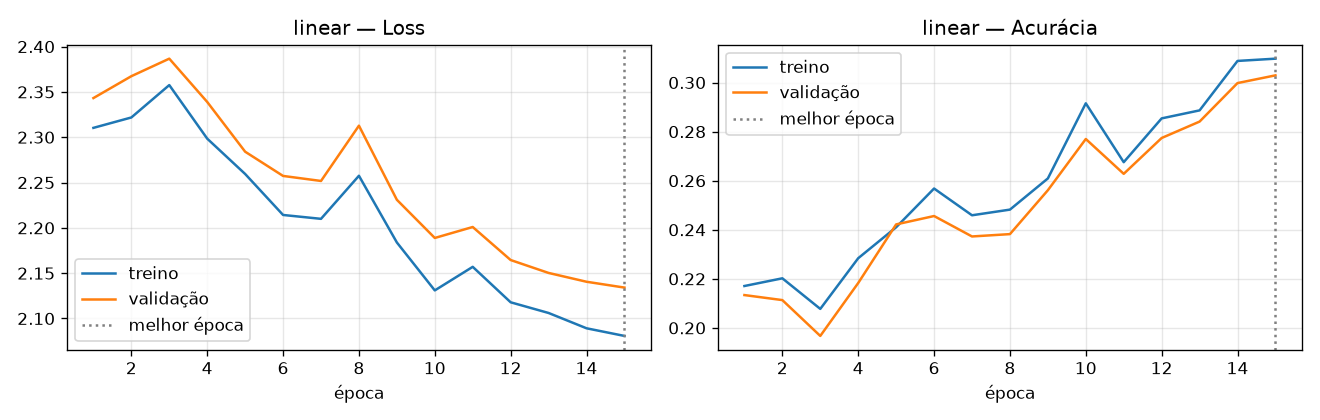
\includegraphics[width=0.78\textwidth]{linear.png}
  \caption{Classificador linear. Treino e validação ficam juntos e baixos (cerca de 30\%): é
  \textbf{underfitting}, porque o modelo não tem capacidade para separar os dígitos.}
  \label{fig:linear}
\end{figure}

\begin{figure}[H]
  \centering
  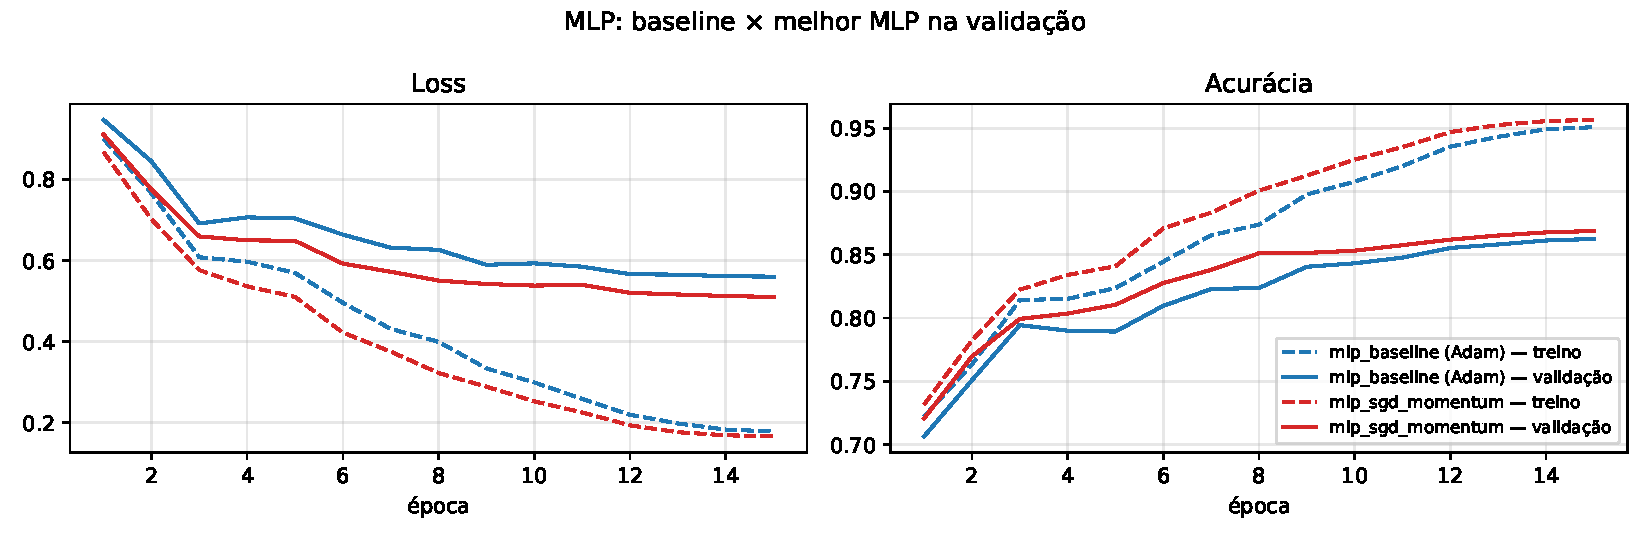
\includegraphics[width=0.9\textwidth]{mlp.pdf}
  \caption{MLP baseline (Adam) e a melhor MLP na validação (SGD com momentum). A loss de treino continua caindo
  enquanto a de validação estabiliza, e a acurácia de treino passa da de validação por cerca de 9 pontos:
  \textbf{overfitting}.}
  \label{fig:mlp}
\end{figure}

\begin{figure}[H]
  \centering
  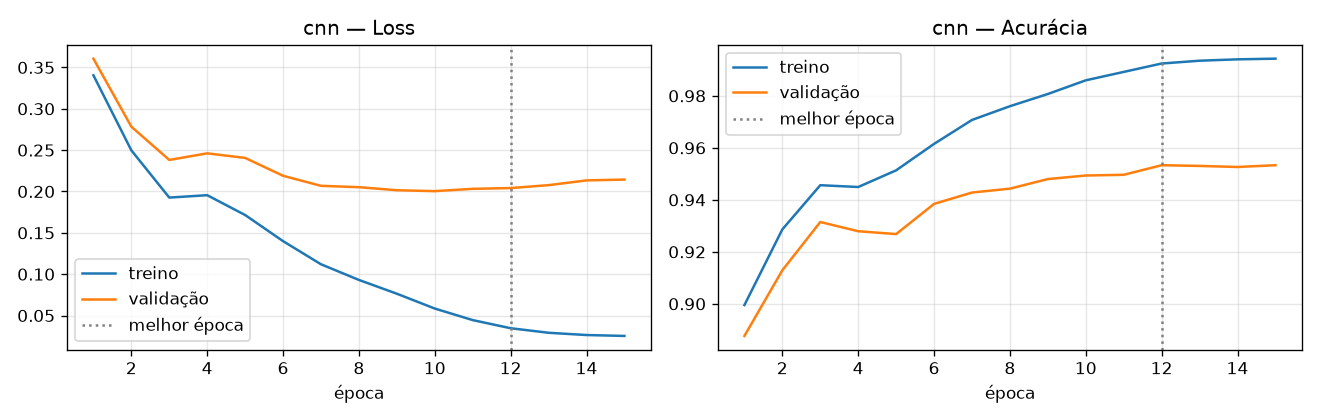
\includegraphics[width=0.78\textwidth]{cnn.png}
  \caption{CNN sem augment. O treino chega perto de 100\%, e a loss de validação atinge o mínimo na época 10 e
  volta a subir: \textbf{overfitting}, que o data augmentation corrige nas versões seguintes.}
  \label{fig:cnn}
\end{figure}

\begin{figure}[H]
  \centering
  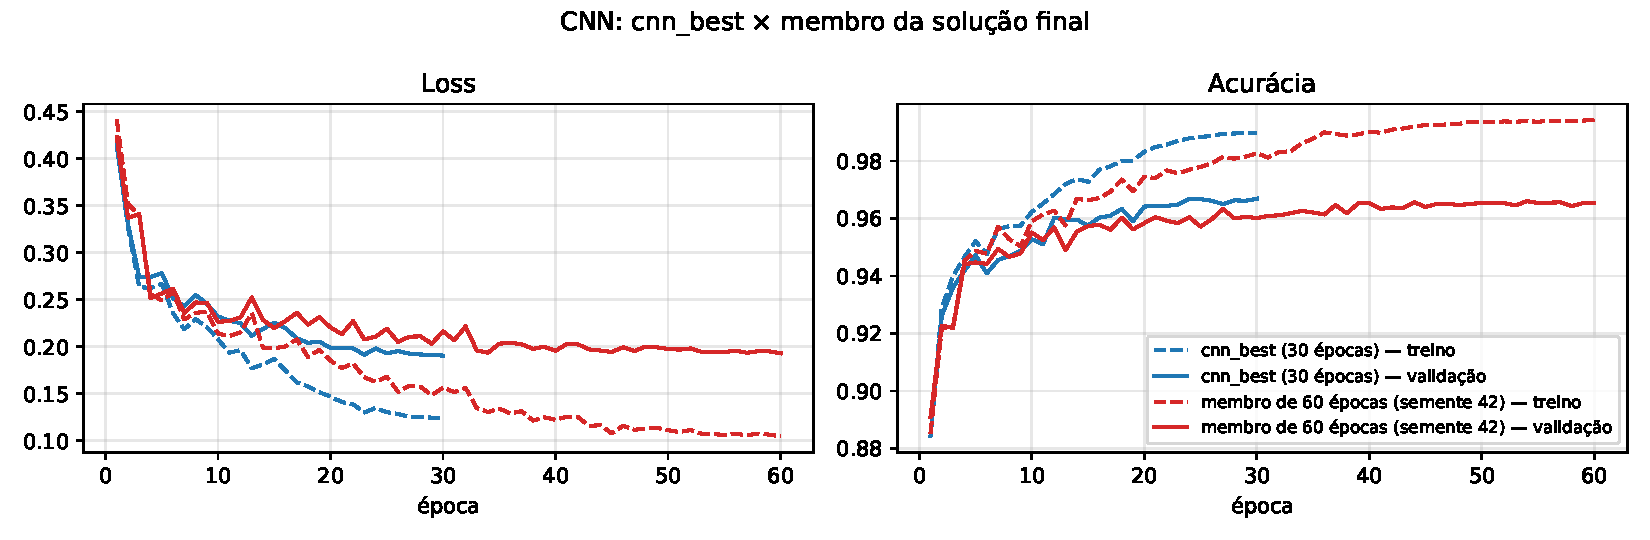
\includegraphics[width=0.9\textwidth]{cnn_best_e60.pdf}
  \caption{A \texttt{cnn\_best} (30 épocas) e um membro da solução final (a mesma CNN, 60 épocas, semente 42).
  Com augment, cutout, weight decay e label smoothing, a diferença entre treino e validação é menor que na
  Figura~\ref{fig:cnn} e a loss de validação não volta a subir. No membro de 60 épocas, as métricas de treino
  são medidas numa amostra fixa de 7.325 imagens do treino.}
  \label{fig:cnnbest}
\end{figure}

\begin{figure}[H]
  \centering
  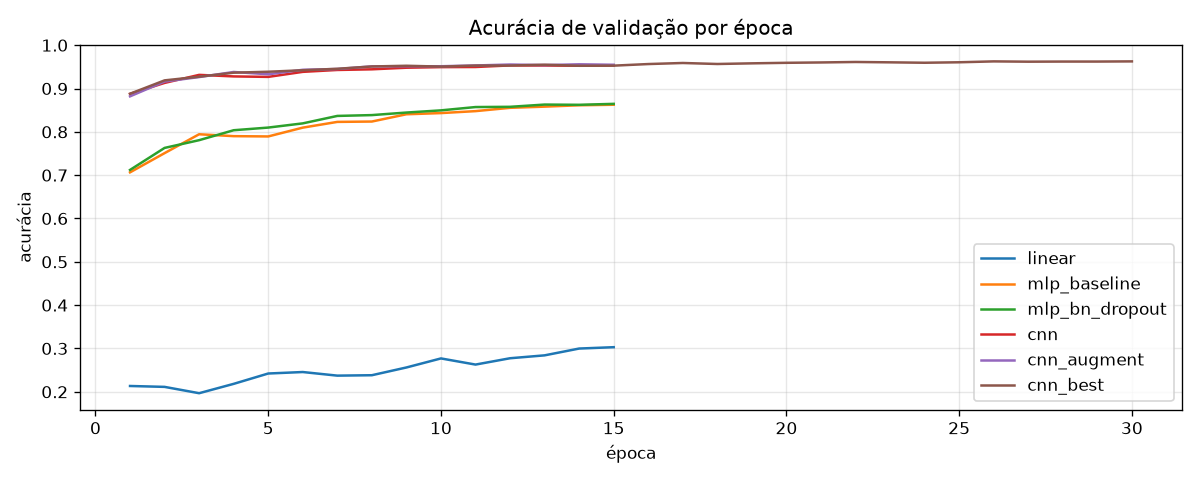
\includegraphics[width=0.7\textwidth]{comparacao_validacao.png}
  \caption{Acurácia de validação por época dos principais modelos.}
  \label{fig:comp}
\end{figure}

\section{Melhor solução}

\paragraph{Arquitetura.} Um ensemble de 20 CNNs iguais à \texttt{cnn\_best}: três blocos de três convoluções
$3\times3$ (32, 64 e 128 filtros) com BatchNorm e ReLU, max pooling depois de cada bloco, e uma camada densa de 256
com Dropout 0,3 antes da saída de 10 classes. Cada CNN tem 1.009.226 parâmetros, e o ensemble, 20.184.520. A
predição é a média do softmax dos 20 modelos na imagem original e em 8 cópias deslocadas 1 e 2 pixels na
horizontal e na vertical (TTA shift12), sem espelhamento.

\paragraph{Hiperparâmetros.} AdamW com taxa de aprendizado $10^{-3}$, weight decay 0,05, decaimento cosseno em 60
épocas, batch 64, label smoothing 0,1, data augmentation geométrico e cutout $8\times8$. As sementes são 42 a 61,
uma por membro, e a divisão é sempre a da semente 42.

\paragraph{Treino final.} Cada membro foi retreinado com todo o \texttt{split="train"} (treino e validação),
como o enunciado permite, e parou na época em que o membro de validação da mesma semente teve a melhor
validação (entre as épocas 40 e 60).

\paragraph{Acurácia.} \textbf{\valFinal{} de validação} (linha 10 da Tabela~\ref{tab:evol}) e \textbf{\testeFinal{}
no teste}. A solução anterior, o ensemble de 5 \texttt{cnn\_best} com TTA, tinha \valEnsCinco{} e
\testeEnsCinco{}, e uma única \texttt{cnn\_best} retreinada, \valCnnBest{} e \testeCnnBestFinal{}.

\paragraph{Motivo da escolha.} Foi a maior acurácia de validação entre todas as soluções testadas, e a regra
de escolha foi registrada antes de ver os resultados. O número de membros é o menor em que a curva de validação
já estabilizou (20; com 25 e 30, não ganha), e o TTA é o melhor na validação com 20 membros. Mais épocas também
ganharam numa segunda divisão, que não guiou nenhuma escolha. O teste foi lido uma única vez, já com a solução
fechada.

{\sloppy
\paragraph{Predições e reprodução.} É este o modelo que gerou o arquivo
\texttt{SAMUEL\_WILKER\_BERNARDO\_\allowbreak RESULTS.txt}: o notebook carrega os pesos dos 20 membros
(\texttt{weights/pt4/}) e classifica automaticamente as 203.856 imagens do conjunto adicional, que nunca foram
usadas no treino nem em nenhuma escolha. As acurácias e as predições se reproduzem exatamente a partir desses
pesos, pelo notebook. Retreinar os membros com as mesmas sementes pelo script reproduz o resultado dentro de
cerca de 0,1 ponto, porque o treino na GPU não é determinístico bit a bit.
\par}

\section{Conclusão}

\paragraph{O que funcionou melhor.} A CNN regularizada, combinada num ensemble. Sozinha, a \texttt{cnn\_best}
chega a \valCnnBest{} de validação; o ensemble de 20 com TTA, a \valFinal{}, e \testeFinal{} no teste.

\paragraph{Maior impacto.} Em ordem: trocar a MLP pela CNN (de \valMlpMelhor{} para \valCnn{}); normalizar a
entrada (sem ela, a MLP perde mais de 30 pontos); usar uma taxa de aprendizado adequada; data augmentation e as
demais regularizações da \texttt{cnn\_best}; e o ensemble com TTA, que reduziu o erro de teste de uma CNN sozinha
em cerca de um quarto. Mudanças de capacidade (filtros mais largos e redes residuais maiores) renderam menos que
regularizar e combinar modelos.

\paragraph{Dificuldades.} Reduzir o overfitting da MLP sem perder acurácia de validação; a instabilidade do
Adam com taxa alta; o custo de treino, já que a solução final tem 20 modelos de 60 épocas, o que nos levou a
treinar vários modelos em paralelo na GPU; separar ganhos reais do ruído entre sementes (cerca de 0,1 ponto), o
que exigiu repetir as melhores mudanças com mais sementes e registrar as regras de decisão antes de ver os
resultados; e diferenças pequenas de predição entre a GPU e o CPU, que tornaram necessário gerar as predições
finais sempre pelo mesmo código.



\end{document}
